\subsection{Windrichtungsgeber}
{\begin{minipage}[b][10cm][t]{0.55\textwidth}
Um die Windrichtung angeben zu können, wurde ein Windrichtungsgeber, wie in Abb. \ref{fig:windrichtungsgeber} gezeigt von MISOL verwendet. Er ist genau wie das Ombrometer und das Anemometer mit Reedkontakten realisiert worden (siehe Abb. \ref{fig:interne_schaltung}). Dafür sind acht Reedkontakte im Kreis angeordnet und jeder hat einen in Serie geschalteten Widerstand von unterschiedlichen Dimensionen. Der Dauermagnet kann, je nach Drehwinkel bis zu zwei Reedkontakte gleichzeitig schließen. Dies erlaubt sechzehn verschiedene Winkelpositionen und somit eine Auflösung von 22.5$^{o}$. Mit einem externen Widerstand $R=10k\Omega$ (siehe Abb. \ref{fig:aussere_beschaltung}) wird eine Spannung generiert, welche dann mit dem ADC des Microcontrollers gelesen werden kann. Der Windrichtungsgeber wird mit einer Speisespannung von $V_{+}=5V$ betrieben. Der Windrichtungsgeber hat einen vierpoligen RJ-11 Anschluss. Zudem hat er auf der unteren Seite noch eine RJ-11 Buchse, bei der das Anemometer direkt angeschlossen werden kann. Wie diese Anschlüsse gemapped sind, wird in der Abb. \ref{fig:interne_schaltung} gezeigt. \\
\end{minipage}}
{\begin{minipage}[b][10cm][t]{0.44\textwidth}
\centering
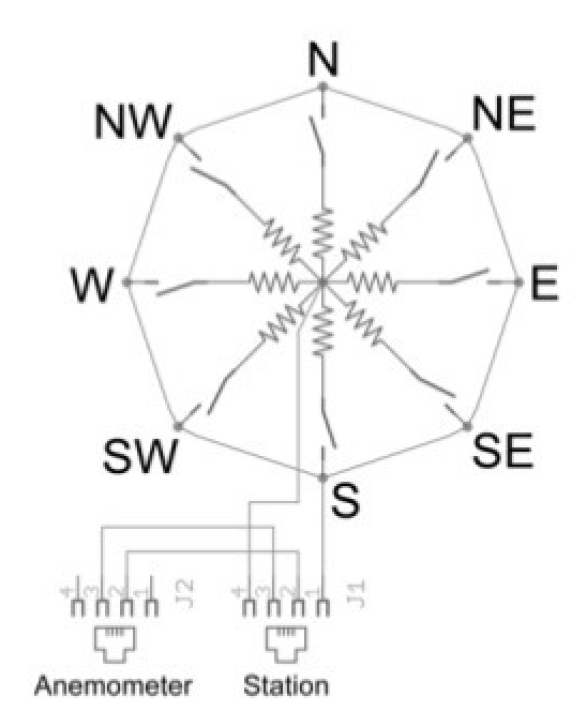
\includegraphics[width=0.9\textwidth]{graphics/windrichtungsgeber/interne_schaltung.PNG}
\captionof{figure}{Interne Schaltung \cite{ADSkeineAngabe}}
\label{fig:interne_schaltung}
\end{minipage}}

\begin{table}[h]
\centering
\caption{Technische Werte \cite{ADSkeineAngabe}}
\begin{tabular}{|c|c|c|c|}
\hline 
Richtung [$^{o}$] & Himmelsrichtung & Widerstand [$\Omega$] & Ausgangsspannung [V] \\ 
\hline 
0 & N & 33k & 3.84 \\ 
\hline 
22.5 &  & 6.57k & 1.98 \\ 
\hline 
45 & NE & 8.2k & 2.25 \\ 
\hline 
67.5 &  & 891 & 0.41 \\ 
\hline 
90 & E & 1k & 0.45 \\ 
\hline 
112.5 &  & 688 & 0.32 \\ 
\hline 
135 & SE & 2.2k & 0.90 \\ 
\hline 
157.5 &  & 1.41k & 0.62 \\ 
\hline 
180 & S & 3.9k & 1.40 \\ 
\hline 
202.5 &  & 3.14k & 1.19 \\ 
\hline 
225 & SW & 16k & 3.08 \\ 
\hline 
247.5 &  & 14.12k & 2.93 \\ 
\hline 
270 & W & 120k & 4.62 \\ 
\hline 
292.5 &  & 42.12k & 4.04 \\ 
\hline 
315 & NW & 64.9k & 4.33 \\ 
\hline 
337.5 &  & 21.88k & 3.43 \\ 
\hline 
\end{tabular} 
\label{tab:technische_werte}
\end{table}

In der Tabelle \ref{tab:technische_werte} sind die Widerstandswerte der in Abb. \ref{fig:interne_schaltung} gezeigten Widerständen und die Werte der Ausgangsspannung bei variabler Winkelposition aufgelistet. Da nun abhängig von der Winkelposition unterschiedliche Widerstände parallel geschalten werden, resultiert am Ausgang eine vom Winkel abhängige Ausgangsspannung.\\

\newpage


{\begin{minipage}[b][6cm][t]{0.49\textwidth}
\centering
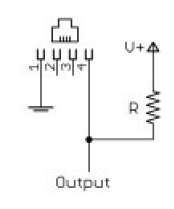
\includegraphics[width=0.5\textwidth]{graphics/windrichtungsgeber/aeussere_beschaltung.PNG} 
\captionof{figure}{Spannungsteiler mit $R=10k\Omega$ \cite{ADSkeineAngabe}}
\label{fig:aussere_beschaltung}
\end{minipage}}
{\begin{minipage}[b][6cm][t]{0.49\textwidth}
\centering
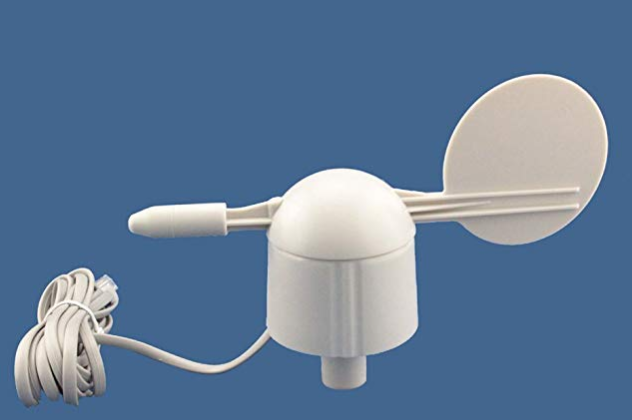
\includegraphics[width=0.9\textwidth]{graphics/windrichtungsgeber/windrichtungsgeber.PNG}
\captionof{figure}{Windrichtungsgeber von MISOL \cite{windrichtungsgeber}}
\label{fig:windrichtungsgeber}
\end{minipage}}

\subsubsection*{Implementation in die Firmware}
Der ADC hat des ATMega2560 hat eine 10 Bit Auflösung und wird mit 5 Volt betrieben. Um das Signal am ADC lesen zu können, wird die Funktion \textit{analogRead()} aufgerufen. Als Rückgabewert wird ein binärer Wert als Dezimalzahl vom Datentyp \textit{float} erhalten. Um diesen Wert in die eigentlich am ADC anliegende Spannung umzurechnen wird die Gleichung \ref{equ:ADC1} umgeformt.
\begin{equation}
\centering
\dfrac{Auflösung ADC}{Betriebsspannung} = \dfrac{analogRead()}{Ausgangsspannung}
\label{equ:ADC1}
\end{equation}
Daraus resultiert:
\begin{equation}
\centering
Ausgangsspannung = \dfrac{analogRead()*Betriebsspannung}{Auflösung ADC}
\label{equ:ADC2}
\end{equation}
Werden nun die Werte in die Gleichung \ref{equ:ADC2} eingefügt, ergibt sich für die Ausgangsspannung $V_{out}$:
\begin{equation}
\centering
V_{out}(analogRead()) = \dfrac{analogRead()*5V}{10}
\label{equ:adc_vout}
\end{equation}
Diese von \textit{analogRead()} abhängige Ausgangsspannung $V_{out}$ wird dann in \textit{if else} Anweisungen zu der Himmelsrichtung zugewiesen und als String abgespeichert.